\section{Half-Giants}
\Quote{Mind of a child, strength of three grown men. I've seen a half-giant tear the walls out of a building because he wanted a better look at the tattoos on a mul inside.}{Daro, human trader}

Legend has it that in ages past, a sorcerer-queen used wizardry to beget a union of giant and human in order to create a race of powerful slaves. Whatever the truth of this legend, the half-giant race has increased in number and is now fairly common especially in human controlled lands near the shore of the Sea of Silt. Half-giants gain great strength, but dull wits, from their giant heritage, and are nearly as agile as their human forbearers.

\begin{figure}[t!]
\centering
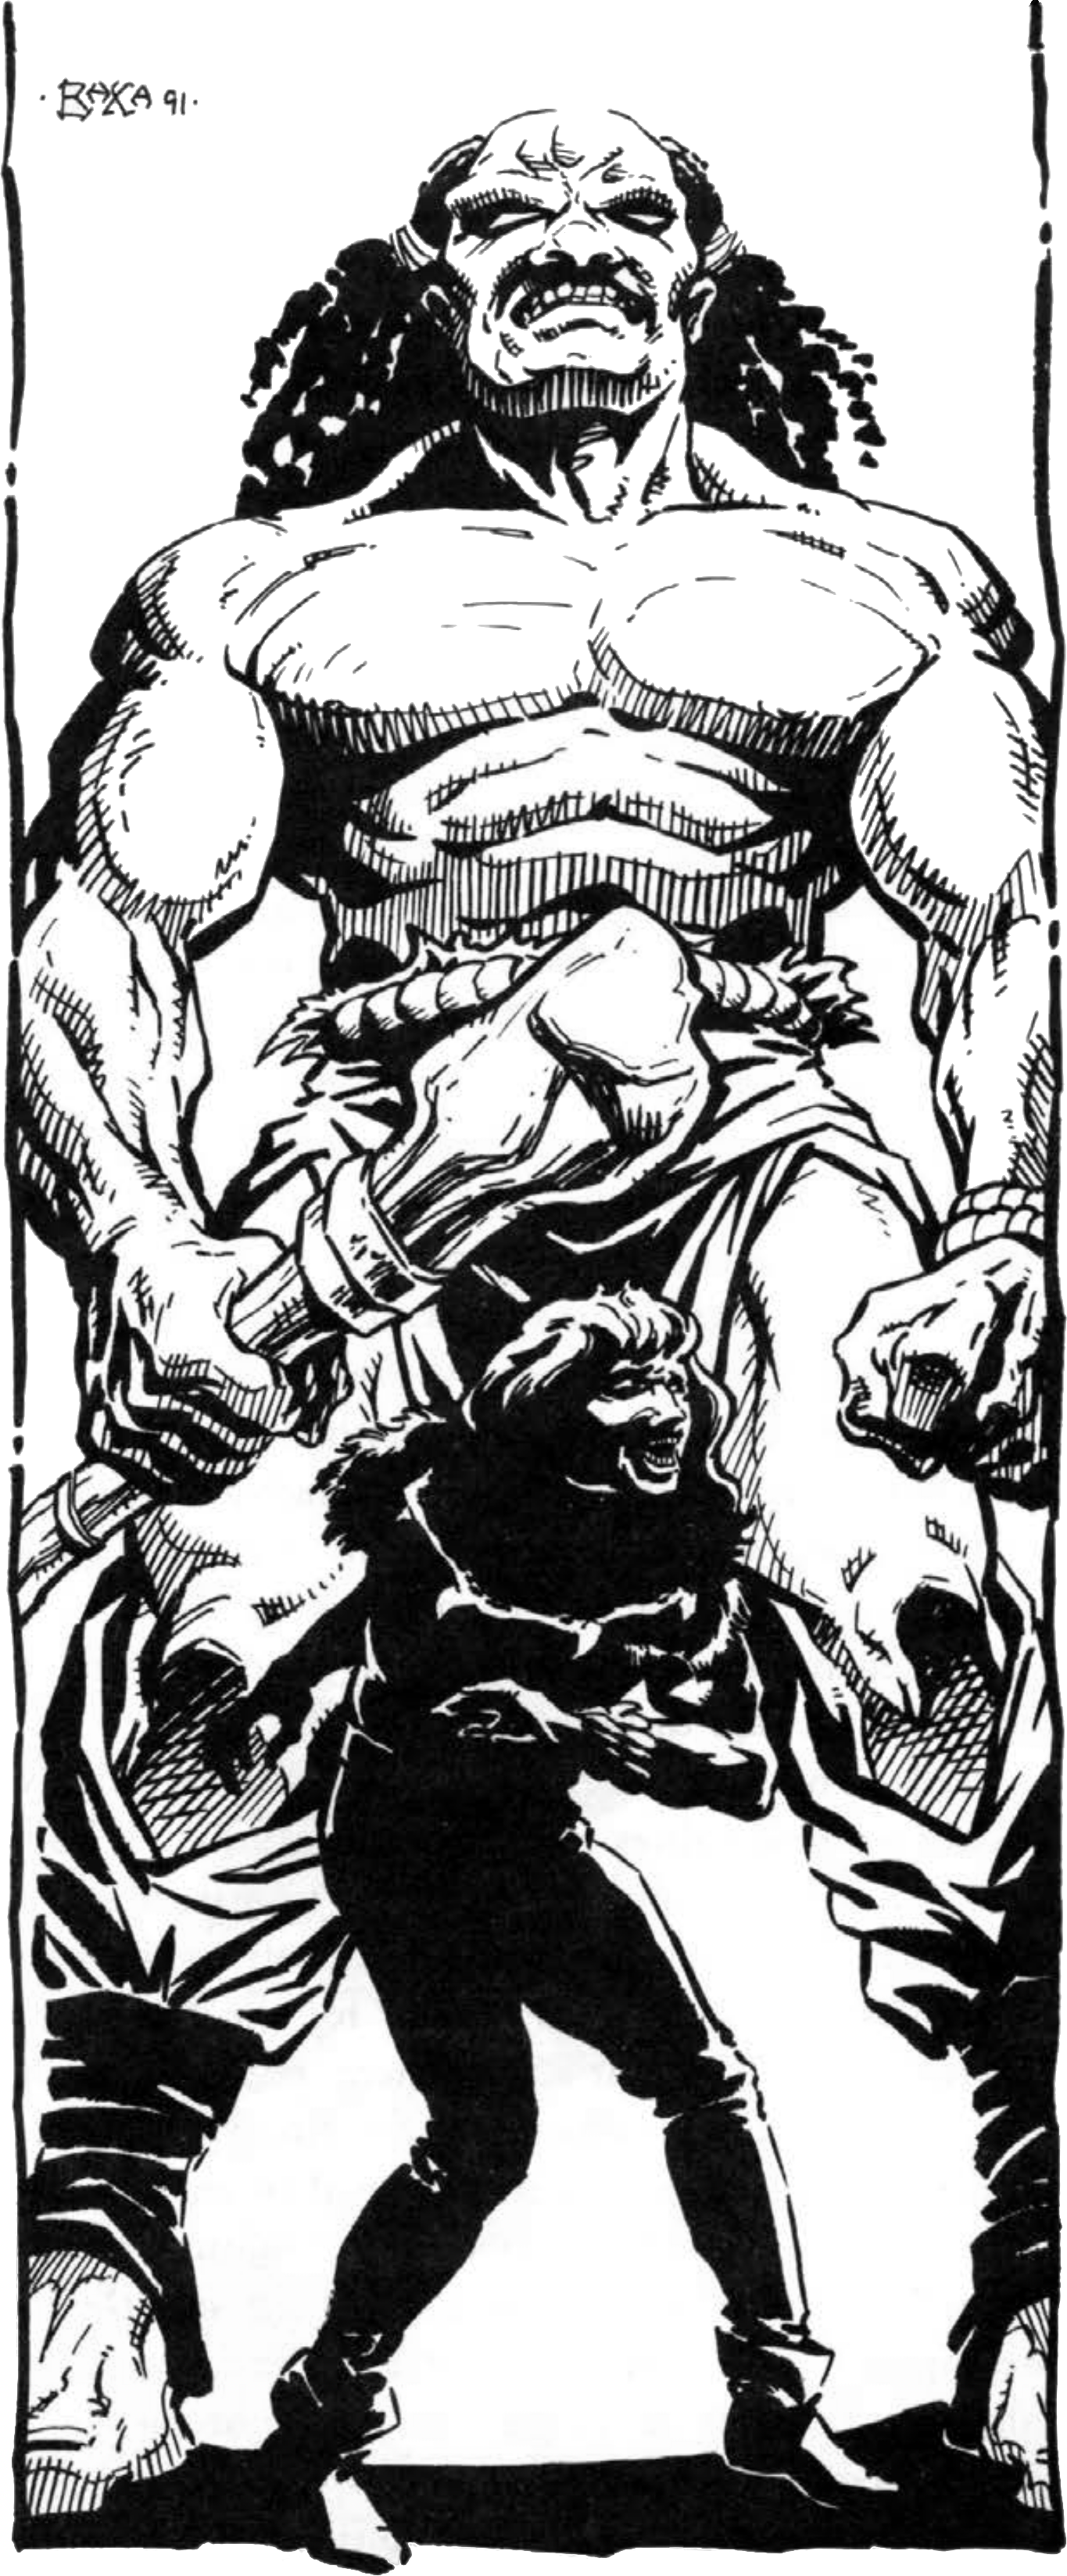
\includegraphics[width=\columnwidth]{images/halfgiant-1.png}
\WOTC
\end{figure}

\textbf{Personality:} Because of their artificial origins, there is no half-giant culture, tradition or homeland. Half-giants readily imitate the customs and cultures of their neighbors. Half-giants often display curiosity, a willingness to learn, and a general tendency towards kindness.

\textbf{Physical Description:} Physically, the half-giant is enormous, standing about 3.5 meters tall and weighing around 600 kg. Half-giants have thick hair, which is often kept braided (especially among females) or in a single tail that hangs behind the head and down the back. They dress in garb suitable to their occupation or environment. Half-giants mature at about 24 years of age and can live about 170 years.

\textbf{Relations:} The most powerful warriors on Athas, half-giants seem content to dwell in humanity's shadow. Half-giants tend to be friendly and eager to please, adopting the lifestyles, skills, and values of those they admire. A half-giant character who encounters a new situation looks around him to see what other people are doing. For example, a half-giant character that happens upon a Dwarven stone quarry may watch the dwarves, and then start quarrying stone himself. If he can make a living at it, he will continue to quarry stone just like his neighbor dwarves do; otherwise he will move on to something else.

\textbf{Alignment:} Half-giants can switch attitudes very quickly, taking on new values to fit new situations. A half-giant whose peaceful farming life is disrupted by marauders may soon adopt the morals of the renegades who sacked his village. A half-giant's nature is to switch his alignment aspect to imitate or otherwise react to a significant change around him.

\textbf{Half-Giant Lands:} Half-giants are most often found in the city-states, serving as gladiators, laborers, soldiers, and guards. A few half-giants collect into wilderness communities, often adopting the culture and customs of neighboring beings. The rare half-giant community often attaches itself to a charismatic or successful leader (not necessarily a half-giant) who demonstrates the tendencies they admire.

\textbf{Magic:} If a half-giant's companions accept wizardry, then the half-giant will also accept it. If a half-giant's companions hate wizardry, then the half-giant will be as eager as anyone to join in stoning a wizard. Among sophisticated companions who accept preserving magic but despise defiling magic, all but the brightest half-giants are likely to become confused, looking to their companions to see how they should react.

\textbf{Psionics:} While a single-classed half-giant psion is very rare, those half-giants take the path of the nomad or of the egoist, becoming killing machines that can take apart a mekillot barehanded.

\textbf{Religion:} Half-giants do not display any affinity for the worship of one element over another.

\textbf{Language:} All half-giants speak the Common speech of slaves. Whatever tongue she speaks, the half-giant's voice is pitched so low as to occasionally be difficult to understand.

\textbf{Names:} Enslaved half-giants often have human names, and because of this they vary greatly. Free half-giants are likely to borrow the naming conventions of the race or people they are imitating at the time their child is born.

\textbf{Adventurers:} Half-giants are usually led to adventure by interesting companions of other races.

\subsection{Half-Giant Society}
A relatively young race, half-giants possess very little cultural identify of their own. Instead they adopt the customs and beliefs of those other cultures in which they live. Because of this, half-giants routinely change their alignment to match those around them who most influence them.
Half-giants can be found from one end of the Tablelands to the other, and often congregate in or near other population centers, absorbing the culture. Rarely do half-giants form communities of their own.

Unlike some other bastard races, half-giants can reproduce. A single off-spring is produced from half-giant unions after almost a year of pregnancy.

Though omnivorous, half-giants are tremendous consumers of water and food. They require twice the amount of food and water than humans. Clothing and equipment need twice the material to construct to fit a half-giant, leading to higher prices for half-giants.

Half-giants tend to damage objects and buildings around them through accidents of size alone. Some considerate half-giants camp outside city walls to avoid causing too much damage, but the draw of a city's culture and the below average intellect of most half-giants limits the number of half-giants who do so.

\subsection{Roleplaying Suggestions}
Always remember how much bigger and heavier you are than everyone else. Take advantage of your height in combat, but remember the disadvantages. Between your size and your lesser wits (even if you are a relatively intelligent half-giant people will assume you to be dull), you find yourself an object of comic relief. You are used to being teased and will endure more witty remarks than most people, but when you have been pushed too far your personality can suddenly shift, and you can unleash astonishing violence on your tormentors and any who stand in your way. Less frequently, these shifts can happen to you without provocation you just wake up with a different ethos and altered disposition.

Remember you are influenced by powerful personalities, and can shift your personality and ethics. You tend to imitate the tactics, clothes and demeanor of your ``little master.''

\subsection{Half-Giant Racial Traits}
\begin{itemize*}
    \item +8 Strength, +4 Constitution, $-4$ Intelligence, $-4$ Wisdom, $-4$ Charisma: Half-giants are renowned for their great strength and dull wits.
    \item Large: As a Large creature, a half-giant takes a $-1$ penalty to Armor Class, a $-1$ penalty on attack rolls, and a $-4$ penalty on \skill{Hide} checks. She gains a +4 size bonus on grapple checks, and her lifting and carrying limits are double those of Medium characters, but she uses bigger weapons than humans use.
    \item Half-giants occupy a space of 3 meters and have a reach of 3 meters.
    \item Humanoid (half-giant): Half-giants are humanoid creatures with the half-giant subtype.
    \item Half-giant base land speed is 12 meters.
    \item Axis Alignment: One aspect of the half-giant's alignment must be fixed, and chosen during character creation. The other half must be chosen when they awake each morning. They are only bound to that alignment until they sleep again. For example, a half-giant may have a fixed lawful alignment. Every morning, he must choose to be lawful good, lawful neutral or lawful evil. This alignment change is not mandatory.
    \item Fit Body: Half-giants double their hit die rolls (but not their Constitution modifier). For example, an 1st-level half-giant barbarian has 24 hit points plus her Constitution modifier.
    \item Half-giants consume double the amount of food and water humans do.
    \item Favored Class: Barbarian. A multiclass half-giant's barbarian class does not count when determining whether he takes an experience point for multiclassing.
    \item Automatic Languages: Common. Bonus Languages: Dwarven, Gith, and Giant. Half-giants will often pick up a race's tongue if imitating them long enough.
    \item Level Adjustment: +2.
\end{itemize*}